\documentclass[a4paper,12pt]{scrartcl}

\newcommand{\dropsign}[1]{\smash{\llap{\raisebox{-.5\normalbaselineskip}{$#1$\hspace{2\arraycolsep}}}}}%

\usepackage[utf8]{inputenc}
\usepackage[ngerman]{babel}
\usepackage{multicol}
\usepackage{scrpage2}\pagestyle{scrheadings}
\usepackage{graphicx} 
\usepackage{tikz}
\usepackage{minted}
\usepackage{pgfplots}
\usepackage{hyperref}
\usepackage{tikz-timing}

\ihead{Blatt 7, G2B}
\chead{Elena Noll, Sven-Hendrik Haase, E. Böhmecke}
\ohead{\today}
\pagestyle{scrheadings}
\setheadsepline{1pt}
\setcounter{secnumdepth}{0}

\begin{document}

\section{Aufgabe 27}
\subsection{a)}
\(d_0\) laesst sich in Bit oder Byte angeben. \(d_c\) laesst sich in Bit bzw. Byte pro Sekunde
angeben.

\subsection{b)}
Wenn \(lim_{t \to 0}\) gilt, dann bleibt als einziges Symbol, das nicht 0 wird, in der Formel
\(d_0\) stehen. Dieses Symbol kann dann beliebig gesetzt werden. D.h., dass der LBAP mit dieser
Annahme beliebig viele Daten erzeugen kann.

\subsection{c)}
Die Datenrate wird mindestens so grosz, wie der groestmoegliche Durchsatz \(d_c\) ueber die gesamte
Ubertragungsdauer. D.h., die Datenrate muss mindestens so gross sein, dass \(d_c * t + d_0\) pro
Zeiteinheit uebertragen werden koennen.

\subsection{d)}
LBAP eignet sich fuer Anwendungen, bei denen eine zu Grunde liegende konstante Uebertragungsrate
durch geringe variable Abweichungen beeinflusst wird. Es eignet sich nicht fuer Anwendungen mit
sehr grossen Abweichungen ueber lange Zeitraeume. Bei Medienuebertragungen von Medien mit bekannten
maximalen Datenraten beispielsweise eignet sich LBAP gut. Diese Medien werden haeufig so encodiert,
dass ihre variable Datenrate minimiert wird, aber einige Intervalle innerhalb der Uebertragung
haben gegebenenfalls ein sehr viel hoeheres Datenaufkommen. Eine Architektur, die LBAP verwendet,
heisst IntServ. IntServ ist ein QoS-System, das haeufig fuer Video- und Audiouebertragungen
verwendet wird.

\subsection{e)}
Wenn alle Sender mit LBAP beschraenkt sind, dann ist auch der gesamte Datenstrom beschraenkt. Die
Parameter sind so zu waehlen, dass der Empfangsbuffer (wenn wir davon ausgehen, dass alle Sender an
einen einzigen Empfaenger senden) so gross ist, dass das maximale Datenaufkommen aller Sender zu
einem Intervall gespeichert werden kann, damit keine Daten verloren gehen. Die reservierte
Datenrate darf ebenfalls nicht geringer sein als das aufakummulierte Datenaufkommen aller Sender.

\section{Aufgabe 28}
\subsection{a)}
DSSS

Vorteile:
\begin{itemize}
	\item Durch Signatur der Spreizsequenz lassen sich andere Signale herausfiltern.Mehrere Signale können auf einer Frequenz übertragen werden und trotzdem auseinander gehalten werden.
	\item Bietet einen gewissen Störungsschutz bei der Übertragung von Information (überträgt redundante Kopien der Information).
\end{itemize}
Nachteile:
\begin{itemize}
	\item Sender und Empfänger müssen zeitlich synchronisiert werden um die Information wieder entschlüsseln zu können
	\item versagt bei starker Störung und schwachem Nutzsignal
\end{itemize}

FHSS

Vorteile:
\begin{itemize}
	\item Geringe Beeinträchtigung eines Störers auf einer festen Frequenz durch „Frequenz-hopping“
	\item Funktioniert trotz eines schwachen Nutzsignals sehr gut und mit mehreren Sendern auf naheliegenden Frequenzen
\end{itemize}
Nachteile:
\begin{itemize}
	\item Kein Schutz vor Störungen, Übertragungsprotokoll muss sicher stellen das beim nächsten Hop die verlorene Information erneut übertragen wird.
	\item Störer verringert die Übertragungsgeschwindigkeit da verlorene Information erneut übertragen werden muss.
\end{itemize}
\subsection{b)}

i)
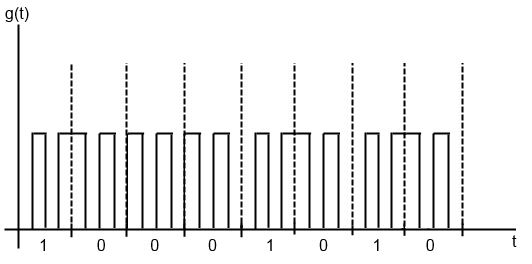
\includegraphics{./aufgabe28bi}

ii)
\begin{center}
  \makebox[\textwidth]{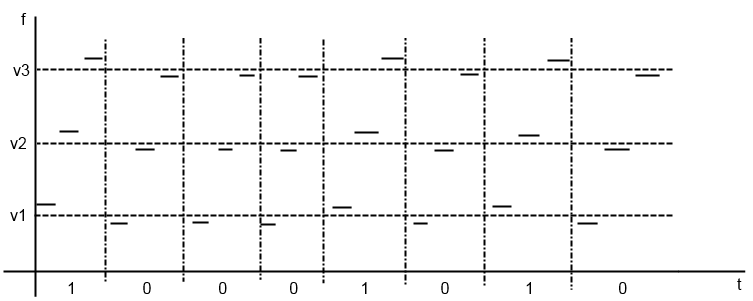
\includegraphics[width=\paperwidth]{./aufgabe28bii}}
\end{center}

\section{Aufgabe 29} 
\subsection{a)}
\subsubsection{i)}
\begin{tikzpicture}
    % horizontal axis
    \draw[->] (0,0) -- (15,0) node[anchor=west] {\(t\)};

    % vertical axis
    \draw[->] (0,0) -- (0,3) node[anchor=south] {Ort};

    % horizontal labels
    \foreach \x in {0,...,14}
        \draw (\x cm,1pt) -- (\x cm,-1pt) node[anchor=north] {\(\x\)};

    % vertical labels
    \draw (1pt, 0) -- (-1pt, 0) node[anchor=east] {S};
    \draw (1pt, 1) -- (-1pt, 1) node[anchor=east] {VR};
    \draw (1pt, 2) -- (-1pt, 2) node[anchor=east] {E};
   
   \draw[step=1,gray,very thin] (0,0) grid (14,2);

    % P_1 (first try)
    \draw[red,thick,->] (0,0) -- (1,1) -- (2,1) -- (3,2) -- (4,2) node[midway,anchor=south] {\(P_1\)};

    % P_2 (first try)
    \draw[blue,thick,->] (2,0) -- (3,1) -- (4,1) node[midway,anchor=north east] {\(P_2\)};

    % SREJ(1)
    \draw[red,thick,dotted,->] (4,2) -- (6,0) node[midway,anchor=south east] {\tiny\(SREJ(1)\)};
    
    % P_3
    \draw[green,thick,->] (4,0) -- (5,1) -- (6,1) -- (7,2) -- (8,2) node[midway,anchor=south] {\(P_3\)};
    
    % P_1 (second try)
    \draw[red,thick,->] (6,0) -- (7,1) -- (8,1) -- (9,2) -- (10,2) node[midway,anchor=south] {\(P_1\)};

    % SREJ(2)
    \draw[blue,thick,dotted,->] (8,2) -- (10,0) node[midway,anchor=north] {\tiny\(SREJ(2)\)};

    % P_2 (second try)
    \draw[blue,thick,->] (10,0) -- (11,1) -- (12,1) -- (13,2) -- (14,2) node[midway,anchor=south] {\(P_2\)};
\end{tikzpicture}
Ankunftszeitpunkt pro Paket: \\
\(P_1\): 10 ZE \\
\(P_2\): 14 ZE \\
\(P_3\): 8 ZE

\subsubsection{ii)}
\begin{tikzpicture}
    % horizontal axis
    \draw[->] (0,0) -- (15,0) node[anchor=west] {\(t\)};

    % vertical axis
    \draw[->] (0,0) -- (0,3) node[anchor=south] {Ort};

    % horizontal labels
    \foreach \x in {0,...,14}
        \draw (\x cm,1pt) -- (\x cm,-1pt) node[anchor=north] {\(\x\)};

    % vertical labels
    \draw (1pt, 0) -- (-1pt, 0) node[anchor=east] {S};
    \draw (1pt, 1) -- (-1pt, 1) node[anchor=east] {VR};
    \draw (1pt, 2) -- (-1pt, 2) node[anchor=east] {E};
   
   \draw[step=1,gray,very thin] (0,0) grid (14,2);

    % P_1 (first try)
    \draw[red,thick,->] (0,0) -- (1,1) -- (2,1) -- (3,2) -- (4,2) node[midway,anchor=south] {\(P_1\)};

    % P_2 (first try)
    \draw[blue,thick,->] (2,0) -- (3,1) -- (4,1) node[midway,anchor=north east] {\(P_2\)};

    % SREJ(1)
    \draw[red,thick,dotted,->] (4,2) -- (6,0) node[midway,anchor=south east] {\tiny\(SREJ(1)\)};
    
    % P_3
    \draw[green,thick,->] (4,0) -- (5,1) -- (6,1) -- (7,2) -- (8,2) node[midway,anchor=south] {\(P_3\)};
    
    % P_1 (second try)
    \draw[red,thick,->] (5,1) -- (6,2) -- (7,2) node[midway,anchor=south] {\(P_1\)};

    % SREJ(2)
    \draw[blue,thick,dotted,->] (4,1) -- (5,0) node[midway,anchor=east] {\tiny\(SREJ(2)\)};
    \draw[blue,thick,dotted,->] (8,2) -- (10,0) node[midway,anchor=east] {\tiny\(SREJ(2)\)};

    % P_2 (second try)
    \draw[blue,thick,->] (5,0) -- (6,1) -- (7,1) -- (8,2) -- (9,2) node[midway,anchor=south] {\(P_2\)};
\end{tikzpicture}
Ankunftszeitpunkt pro Paket: \\
\(P_1\): 7 ZE \\
\(P_2\): 9 ZE \\
\(P_3\): 8 ZE

\subsection{b)}
Es kann vorkommen, dass der Empfaenger zusaetzliche ueberfluessige SREJs
durch das Netz schickt, obwohl sich die angeforderten Pakete bereits auf dem
Weg befinden, ein Beispiel hierfuer sieht man in dem oberen Diagramm. Dadurch
entsteht zusaetzliche Belastung auf dem Netzwerk. Zusaetzlicher Aufwand entsteht
ebenfalls dadurch, dass der VR die ganzen Pakete zwischenspeichern muss,
wenn der E sie anfordert. Das erhoeht die Komplexitaet.\\
End-to-End-Kontrolle ist in der Regel dann guenstiger, wenn die Verbindung sehr
stabil ist, denn dann muss von dem Speicher des VR kaum Gebrauch gemacht werden.\\
Da Node-to-Node-Kontrolle transitiv auch End-to-End-Kontrolle beeinhaltet
(zumindest laut Aufgabenstellung), kann auf eine zusaetzliche End-to-End-Kontrolle
verzichtet werden.

\subsection{c)}
Mit folgendem einfachen Python3 Code habe ich die nachfolgenden Werte ermittelt

\begin{minted}[linenos,fontsize=\footnotesize]{python}
#!/usr/bin/env python3

import random

chances_of_failure = [1, 5, 10, 25, 50, 75, 98, 99]

for chance in chances_of_failure:
    tries_list = []
    for i in range(1000000):
        tries = 0
        success = False

        # Try transfer until it succeeds
        while not success:
            if random.randint(0, 100) < chance:
                # Failure
                tries += 1
            else:
                # Success
                success = True

                # Put number of attempts into list so we can calculate average
                tries_list.append(tries)

    average = sum(tries_list) / float(len(tries_list))
    print("Average number of tries for {}% failure chance: {}".format(chance, average))

\end{minted}

\begin{verbatim}
Average number of tries for 1% failure chance: 0.010017
Average number of tries for 5% failure chance: 0.052015
Average number of tries for 10% failure chance: 0.109774
Average number of tries for 25% failure chance: 0.328764
Average number of tries for 50% failure chance: 0.982926
Average number of tries for 75% failure chance: 2.887324
Average number of tries for 98% failure chance: 32.612025
Average number of tries for 99% failure chance: 49.486482
\end{verbatim}

\end{document}

